\section{Panoramica di possibili diverse architetture per Android Real-Time}
\subsection{Proposte ad alto livello}
\begin{figure}[h]
	\centering
	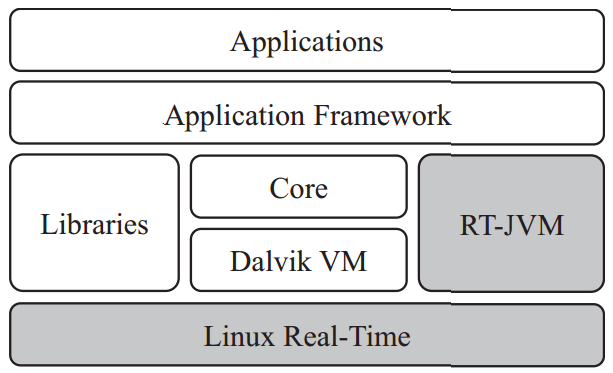
\includegraphics[width=0.7\linewidth]{androidPienoSupportoRT}
	\caption{Android Full real-time}
	\label{fig:androidpienosupportort}
\end{figure}
Una prima soluzione è mostrata in Figura~\ref{fig:androidpienosupportort} e considera la sostituzione di Linux con una versione real-time e l'aggiunta di una RT VM. Queste modifiche aggiungono prevedibilità e determinismo, ed è inoltre possibile aggiungere nuove politiche di scheduling attraverso le classi di scheduling e migliori strategie di gestione delle risorse. D'altra parte, però, tutti i driver utilizzati dal dispositivo devono essere implementati in un ottica real-time, e questo può portare a sforzi non necessari. La seconda modifica proposta riguarda l'aggiunta di una RT VM. Questa è considerata vantaggiosa, perché permette una gestione della memoria prevedibile. Inoltre, a seconda dell'algoritmo utilizzato, è anche possibile ottenere uno scheduling real-time, migliori meccanismi di sincronizzazione ed evitare l'inversione di priorità. Queste aggiunte sono assolutamente necessarie se si vuole ottenere una VM deterministica e prevedibile. Quest'ultima interagisce direttamente con il kernel per funzionalità come scheduling e gestione dei limiti di memoria. Non è necessario tenere il passo con le versioni di Android, perché è presente anche la DVM, ma è necessario implementare, la prima volta, una nuova Vm da zero e l'interprete Dalvik. Inoltre l'interazione di due VM può essere problematica, e può essere necessario pensare a nuovi algoritmi per ottimizzare lo scheduling.

\begin{figure}[h]
	\centering
	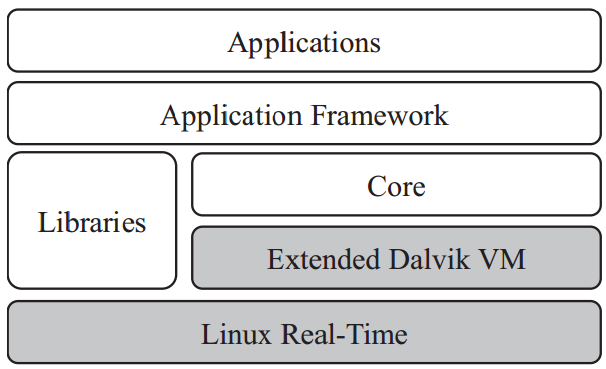
\includegraphics[width=0.7\linewidth]{androidEstesoRT}
	\caption{Android esteso con funzionalità real-time}
	\label{fig:androidestesort}
\end{figure}
La seconda soluzione è quella di sostituire Linux una versione real-time e di aggiungere funzionalità real-time a DVM (Figura~\ref{fig:androidestesort}). I vantaggi e gli svantaggi della sostituzione di Linux sono uguali a prima. Ora però la DVm viene estesa per supportare RTSJ. Questo permette di aggiungere alla DVm tutte le caratteristiche real-time previste dalla RTSJ, come GC real-time e gestione asincrona di eventi. In questo caso è però necessario stare al passo con i rilasci di nuove versioni della VM, per poter portare le modifiche a tutti i dispositivi Android.

\begin{figure}[h]
	\centering
	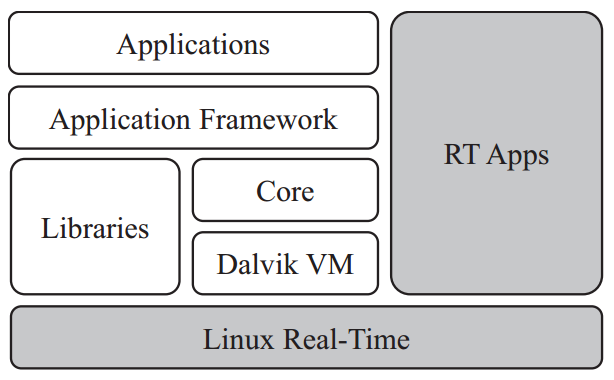
\includegraphics[width=0.7\linewidth]{rtandroidParziale}
	\caption{Android con support real-time parziale}
	\label{fig:rtandroidparziale}
\end{figure}
Il terzo approccio (Figura~\ref{fig:rtandroidparziale}) si basa ancora su Linux real-time e utilizza applicazioni real-time direttamente sopra il sistema operativo, utilizzando le librerie native. Questo è un vantaggio per quelle applicazioni che non necessitano della VM. Al contrario, però, le applicazioni che hanno bisogno della VM non possono avere supporto real-time.

\begin{figure}[h]
	\centering
	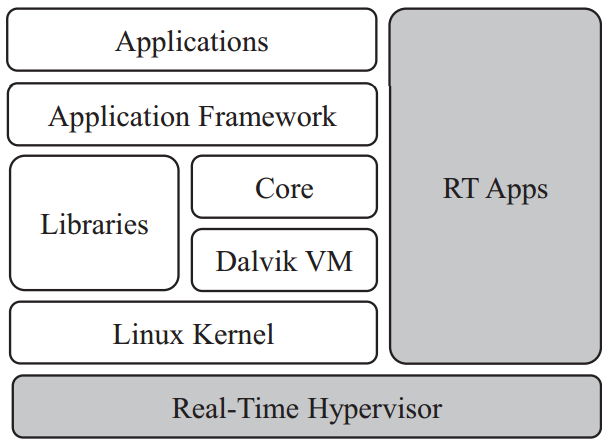
\includegraphics[width=0.7\linewidth]{androidConRTHypervisor}
	\caption{Android con real-time hypervisor}
	\label{fig:androidconrthypervisor}
\end{figure}
Il quarto approccio (Figura~\ref*{fig:androidconrthypervisor}) utilizza un real-time hypervisor in grado di eseguire parallelamente Android e applicazioni real-time. Questa soluzione è simile a quella utilizzata da alcuni sistemi operativi real-time, come RTLinux, e consiste nell'eseguire task real-time parallelamente (ma con priorità maggiore) a task del kernel. Lo svantaggio è che le applicazioni real-time godono delle sole funzionalità offerte dall'hypervisor, e quindi non possono utilizzare né i servizi della DVM né quelli di Linux. Inoltre, se un'applicazione real-time si blocca, l'intero sistema potrebbe bloccarsi.

\subsection{Liberare manualmente la memoria}
In \ref{sec:gcandroid} sono stati spiegate alcune criticità della GC in Android. Tuttavia, disabilitarla completamente non è una strada percorribile. Ogni processo ha la sua area di memoria e il GC viene invocato quando non c'è posto per soddisfare una richiesta di allocazione. Non liberare la memoria in questo contesto porterebbe sicuramente a comportamenti non prevedibili e distruttivi. Una soluzione più promettente potrebbe essere quella di liberare manualmente la memoria. In questo modo la probabilità che il GC sia invocato (e di conseguenza che l'applicazione venga bloccata) è minore. 

\begin{figure}[h]
	\centering
	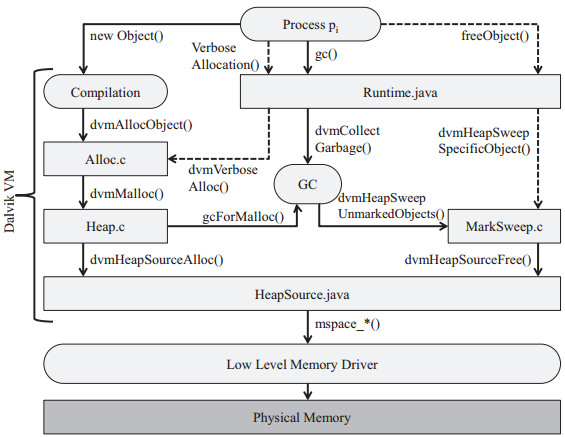
\includegraphics[width=0.7\linewidth]{../images/androidMemoryManagement}
	\caption{Gestione della memoria in Android}
	\label{fig:androidmemorymanagement}
\end{figure}

In Figura~\ref{fig:androidmemorymanagement} è mostrata la gestione della memoria in Android. Le transizioni rappresentano eventi di sistema, come chiamate di metodi, e mostrano i file sorgente coinvolti. I rettangoli arrotondati indicano entità astratte e componenti di sistema. Le linee tratteggiate rappresentano le estensioni proposte in questa soluzione. 

Durante la compilazione di un'applicazione Android, ogni istanziazione (\texttt{new}) viene tradotta in una chiamata a \texttt{dvmAllocObject()}. Questo metodo prende come argomento un riferimento alla classe richiesta. Tra le altre cose, questo riferimento contiene la dimensione dell'oggetto che si vuole creare. La dimensione viene passata a \texttt{dvmMalloc()}, che alloca la quantità di memoria desiderata. In generale, quest'ultima è responsabile della gestione degli errori, mentre l'allocazione vera e propria viene fatta da \texttt{dvmHeapSourceAlloc()}, che ritorna il risultato senza nessuna validazione. Se non ci sono errori, blocco viene poi convertito nell'oggetto e l'esecuzione continua. La chiamata può però fallire, ritornando un puntatore nullo e indicando la situazione della memoria. A questo punto \texttt{dvmMalloc()} prova a risolvere il problema avviando il GC,l dopodiché l'allocazione viene ripetuta o viene lanciata un'eccezione (\texttt{OutOfMemoryException}). Gli oggetti che non sono marcati dopo la passata del GC sono eliminabili. L'eliminazione viene fatta da \texttt{dvmHeapSweepUnmarkedObjects()}, che rilascia la memoria chiamando \texttt{dvmHeapSourceFree()} per ogni riferimento. Android offre anche la possibilità di richiedere esplicitamente la passata del GC, chiamando \texttt{Runtime.gc()} manualmente. Le chiamate esplicite al GC hanno gli stessi effetti negativi di quelle implicite. L'idea è quindi quella di pulire la memoria manualmente, oggetto per oggetto senza chiamare il GC. Sappiamo che \texttt{dvmHeapSourceFree()} offre la possibilità di eliminare un oggetto, dato il suo riferimento. Viene quindi aggiunto alla DVM un nuovo metodo, \texttt{dvmHeapSweepSpecificObject()}, che chiama \texttt{dvmHeapSourceFree()}. In più la classe \texttt{Runtime} viene estesa con il metodo \texttt{freeObject()}, per rendere disponibile la funzionalità per le applicazioni Android. \texttt{freeObject()} riceve come argomento un oggetto da rimuovere. Calcola il puntatore al blocco che contiene l'oggetto e lo passa a \texttt{dvmHeapSweepSpecificObject()}, che lo rimuove attraverso \texttt{dvmHeapSourceFree()}. Dopodiché la memoria è disponibile per un'altra allocazione. Uno svantaggio è che \texttt{freeObject()} può essere usato solo per quegli oggetti di cui lo sviluppatore è al corrente, ma la memoria può anche essere riempita di oggetti temporanei. Una soluzione è quella di aggiungere a \texttt{Runtime} anche il metodo \texttt{verboseAllocations()}, che permette di avere dei log su tutti gli oggetti che vengono allocati durante la vita di un processo. Questo log può poi essere usato per rendersi conto degli oggetti creati e liberare la memoria di conseguenza. 

\subsubsection{Valutazione}
In Figura~\ref{fig:valutazionegestionemanualememoria} viene mostrato un confronto fra la gestione della memoria manuale e con GC. Si nota che, raggiunti più o meno i 2900kB di memoria riferita, la DVM invoca il GC e l'applicazione viene, conseguentemente, bloccata. Al contrario, con la gestione manuale, il GC non viene mai invocato, perché la memoria riferita resta sempre sotto la soglia.
\begin{figure}[h]
	\centering
	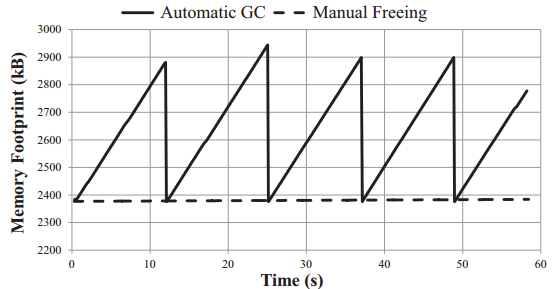
\includegraphics[width=0.7\linewidth]{valutazioneGestioneManualeMemoria}
	\caption{Valutazione della soluzione}
	\label{fig:valutazionegestionemanualememoria}
\end{figure}

Lo svantaggio e il limite evidente di questo approccio è che richiede che i programmatori gestiscano manualmente la memoria, proprio come in C o C++. Questo processo è estremamente difficoltoso, e può portare a molti leak e a gestioni scorrette. Sebbene prevenga l'invocazione del GC, gli errori introdotti dalla gestione manuale potrebbero portare l'applicazione ad un fallimento.